\input{../Preambulos/preambulo_materiales}
\usepackage[siunitx]{circuitikz}
\usetikzlibrary{patterns, arrows}
\usetikzlibrary{decorations.markings}
\usetikzlibrary{matrix}

\title{Ejercicios del Examen Tema 4 \\ {\large Curso Física Computacional}}
\author{M. en C. Gustavo Contreras Mayén. \texttt{gux7avo@ciencias.unam.mx}}

\date{ }
\begin{document}

\maketitle
\fontsize{14}{14}\selectfont

A continuación se presenta la lista de ejercicios a resolver que conforman la parte de la evaluación del Tema 4, que completa el segundo examen parcial, con la finalidad de brindar más tiempo en la solución de los problemas se entrega anticipadamente la lista de ejercicios.
\par
Cada ejercicio tiene una calificación de un punto siempre y cuando esté debidamente resuelto, se ocupará la rúbrica de evaluación que ya conoces.
\par
Revisa cuidadosamente cada ejercicio, ya que deberás de mencionar qué técnica de solución has elegido y justificar su uso, en caso de que el problema indique expresamente la técnica a utilizar, no será necesario que lo expliques.

\begin{enumerate}
\item Los dos péndulos están conectados por un resorte que no se deforma cuando los péndulos están verticales.
\begin{figure}[H]
\centering
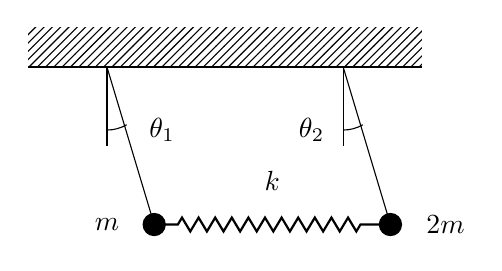
\begin{tikzpicture}
    \tikzstyle{spring}=[thick,decorate,decoration={zigzag,pre length=0.3cm,post
  length=0.3cm,segment length=6}]
	\draw (0,0) [pattern = north east lines, draw = none] rectangle (5,0.5);
    \draw (0, 0) -- (5, 0);
    \draw (1, 0) -- (1, -1);
    \draw (1, 0) -- (1.6, -2);
    \draw (1, -0.8) arc (270:300:0.5);
    \node at (1.7, -0.8) {$\theta_{1}$};
    \draw [fill] (1.6, -2) circle (4pt);
    \node at (1, -2) {$m$};
    \draw (4, 0) -- (4, -1);
    \draw (4, 0) -- (4.6, -2);
    \draw (4, -0.8) arc (270:300:0.5);
    \node at (3.6, -0.8) {$\theta_{2}$};
    \draw [fill] (4.6, -2) circle (4pt);
    \node at (5.3, -2) {$2m$};

    \draw [spring](1.6, -2) -- (4.6, -2) node [midway, above=0.3cm] {$k$}; 
\end{tikzpicture}
\end{figure}

Se puede demostrar que las ecuaciones de movimiento del sistema son:
\begin{align*}
k \, L (\theta_{2} - \theta_{1}) - m \, g \, \theta_{1} &= m \, L \, \ddot{\theta}_{1} \\[0.5em]
-k \, L (\theta_{2} - \theta_{1}) - 2 \, m \, g \, \theta_{2} &= m \, L \, \ddot{\theta}_{2}
\end{align*}
donde $\theta_{1}$ y $\theta_{2}$ son los desplazamientos angulares y $k$ es la rigidez del resorte. 

Calcula las frecuencias angulares de vibración y las amplitudes relativas de los desplazamientos angulares. Utiliza $m = \SI{0.25}{\kilo\gram}$, $k = \SI{20}{\newton\per\metre}$, $L = \SI{0.75}{\meter}$ y $g = \SI{9.80665}{\meter\per\square\second}$.
\item Considera el siguiente circuito eléctrico:
\begin{figure}[H]
    \centering
    \begin{circuitikz}
	    \draw (0, 3) to [cC, l=$C$] (0, -3);
        \draw (0, 3) to [L, l=$L$] (3, 3);
        \draw (3, 3) to [L, l=$L$] (6, 3);
        \draw (3, 3) to [cC, l_=$C$] (3, 0);
        \draw (6, 3) -- (6, 0) -- (3, 0);
        \draw (3, 0) to [cC, l=$C$] (3, -3);
        \draw (0, -3) -- (3, -3);
        \draw (3, -3) to [L, l=$L$] (6, -3);
        \draw (6, -3) -- (6, 0);
        
        \draw [-stealth, color=red, thick] (1, 2.5) -- (0.4, 2.5) -- (0.4, 1.) node [right] {$i_{1}$};
        \draw [-stealth, color=red, thick] (1.52, -2.5 ) -- (2.6, -2.5) -- (2.6, -2) node [left] {$i_{1}$};

        \draw [-stealth, color=red, thick] (4.2, 2.5) -- (3.6, 2.5) -- (3.6, 1.4) node [right] {$i_{2}$};
        \draw [-stealth, color=red, thick] (4.8, 0.6) -- (5.6, 0.6) -- (5.6, 1.2) node [left] {$i_{2}$};
        
        \draw [-stealth, color=red, thick] (4.4, -0.4) -- (3.8, -0.4) -- (3.8, -1.2) node [right] {$i_{3}$};
        \draw [-stealth, color=red, thick] (5, -2.6) -- (5.6, -2.6) -- (5.6, -1.8) node [left] {$i_{3}$};

    \end{circuitikz}
\end{figure}
La ley de Kirchoff para la corriente nos dice que:
\begin{align*}
3 \, i_{i} - i_{2} - i_{3} &= - L \, C \, \dv[2]{i_{1}}{t} \\[0.5em]
-i_{i} + i_{2} &= - L \, C \, \dv[2]{i_{2}}{t} \\[0.5em]
-i_{i} + i_{3} &= - L \, C \, \dv[2]{i_{3}}{t}
\end{align*}
Calcula las frecuencias angulares del circuito y las amplitudes relativas de las corrientes en las mallas.
\item Para la siguiente matriz:
\begin{align*}
\vb{A} =
\begin{bmatrix}
4 & -2 & 1 & -1 \\
-2 & 4 & -2 & 1 \\
1 & -2 & 4 & -2 \\
-1 & 1 & -2 & 4
\end{bmatrix}
\end{align*}
\begin{enumerate}
\item Calcula los eigenvalores y eigenvectores con el método de Jacobi.
\item Con el método de la potencia calcula el eigenvalor más grande y el correspondiente eigenvector.
\item Con el método de la potencia calcula el eigenvalor más pequeño y su correspondiente eigevector.
\end{enumerate}
\item Una columna simplemente apoyada como se muestra en la figura (a) consta de tres segmentos con las rigideces a la flexión que se indican.
\begin{figure}[H]
\centering
\begin{tikzpicture}
    \draw (0, 0) rectangle (1.5, 0.3);
    \node at (0.75, 0.8) {$\dfrac{L}{4}$};
    \draw (1.5, -0.2) rectangle (4.5, 0.5);
    \node at (3, 1) {$\dfrac{L}{2}$};
    \draw (4.5, 0) rectangle (6, 0.3);
    \node at (5.2, 0.8) {$\dfrac{L}{4}$};
    \draw (-0.3, -0.5) [pattern = north east lines, draw = none] rectangle (0.3, -0.3);
    \draw (-0.3, -0.3) -- (0.3, -0.3);
    \draw (0, 0) -- (-0.1, -0.3);
    \draw (0, 0) -- (0.1, -0.3);

    \draw (5.7, -0.5) [pattern = north east lines, draw = none] rectangle (6.3, -0.3);
    \draw (5.7, -0.3) -- (6.3, -0.3);
    \draw (6, -0.18) circle (4pt);

    \node at (0.8, -0.3) {$E I_{0}$};
    \node at (3, -0.4) {$2 E I_{0}$};
    \node at (5.2, -0.3) {$E I_{0}$};

    \draw [-stealth, thick] (-1, 0.15) -- (0, 0.15) node [left, pos=-0.1] {$P$};
    \draw [stealth-, thick] (6, 0.15) -- (7, 0.15) node [right, pos=0.9] {$P$};
\end{tikzpicture}
\caption{(a)}
\label{fig:figura_a}
\end{figure}
Si solo interesa el primer modo de flexión, es suficiente modelar la mitad de la viga como se muestra en la figura (b).
\begin{figure}[H]
\centering
\begin{tikzpicture}
    \draw (0, 0) rectangle (5, 0.5);
    \draw (5, -0.1) rectangle (10, 0.6);

    \foreach \x in {1, 2, 3, 4}
        \draw (\x, 0) -- (\x, 0.5);

    \foreach \x in {6, 7, 8, 9}
        \draw (\x, -0.1) -- (\x, 0.6);
    
    \foreach \x in {0,1,...,9,10}
        \node at (\x, -0.3) {$\x$};
    
    \foreach \x in {2.5, 7.5}
        \node at (\x, 1.2) {$\dfrac{L}{4}$};

\end{tikzpicture}
\caption{(b)}
\label{fig:figura_b}
\end{figure}
La ecuación diferencial para el desplazamiento lateral $u (x)$ es:
\begin{align*}
\sderivada{y} = - \dfrac{P}{E \, I} \, u
\end{align*}
con las condiciones de frontera $u (0) = \pderivada{u} (0) = 0$. Las correspondientes ecuaciones en diferencias finitas son:
\begin{align*}
\begin{bmatrix}
2 & -1 & 0 & 0 & 0 & 0 & 0 & \ldots & 0 \\
- 1 & 2 & -1 & 0 & 0 & 0 & 0 & \ldots & 0 \\
0 & - 1 & 2 & -1 & 0 & 0 & 0 & \ldots & 0 \\
0 & 0 & - 1 & 2 & -1 & 0 & 0 & \ldots & 0 \\
0 & 0 & 0 & - 1 & 2 & -1 & 0 & \ldots & 0 \\
0 & 0 & 0 & 0 & - 1 & 2 & -1 & \ldots & 0 \\
\vdots & \vdots & \vdots & \vdots & \vdots & \ddots & \ddots & \ddots & \vdots \\
0 & \ldots & 0 & 0 & 0 &  0 & - 1 & 2 & -1 \\
0 & \ldots & 0 & 0 & 0 &  0 & 0 & -1 & 1
\end{bmatrix}
\begin{bmatrix}
u_{1} \\
u_{2} \\
u_{3} \\
u_{4} \\
u_{5} \\
u_{6} \\
\vdots \\
u_{9} \\
u_{10}
\end{bmatrix}
= \lambda \, 
\begin{bmatrix}
u_{1} \\
u_{2} \\
u_{3} \\
u_{4} \\
u_{5}/1.5 \\
u_{6}/2 \\
\vdots \\
u_{9}/2 \\
u_{10}/4
\end{bmatrix}
\end{align*}
donde:
\begin{align*}
\lambda = \dfrac{P}{E \, I_{0}} \left( \dfrac{L}{20} \right)^{2}
\end{align*}
Escribe un programa que calcule la carga de flexión más baja $\vb{P}$ de la columna con el método de potencia inversa. Utiliza la forma con bandas de las matrices.
\item Se tiene un sistema masa-resorte:
\begin{figure}[H]
\centering
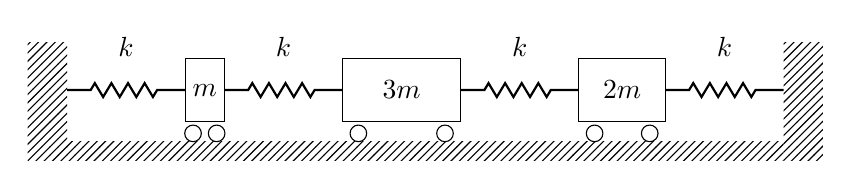
\begin{tikzpicture}
    \tikzstyle{spring}=[thick,decorate,decoration={zigzag,pre length=0.3cm,post
  length=0.3cm,segment length=6}]
    \draw (0, 0) [pattern = north east lines, draw = none] rectangle (9.1, 0.25);
    \draw (0, 0) [pattern = north east lines, draw = none] rectangle (-0.5, 1.5);
    \draw (9.1, 0) [pattern = north east lines, draw = none] rectangle (9.6, 1.5);

    \draw [spring](0, 0.9) -- (1.5, 0.9) node [midway, above=0.3cm] {$k$};
    \draw (1.5, 0.5) rectangle (2, 1.3) node [pos=0.5] {$m$};
    
    \foreach \x in {1.6, 1.9, 3.7, 4.8, 6.7, 7.4}
        \draw (\x, 0.35) circle (3pt);
    
    \draw [spring](2, 0.9) -- (3.5, 0.9) node [midway, above=0.3cm] {$k$};
    \draw (3.5, 0.5) rectangle (5, 1.3) node [pos=0.5] {$3m$};
    \draw [spring](5, 0.9) -- (6.5, 0.9) node [midway, above=0.3cm] {$k$};
    \draw (6.5, 0.5) rectangle (7.6, 1.3) node [pos=0.5] {$2m$};
    \draw [spring](7.6, 0.9) -- (9.1, 0.9) node [midway, above=0.3cm] {$k$};
\end{tikzpicture}
\end{figure}
Las ecuaciones diferenciales de movimiento de ese sistema son:
\begin{align*}
k (- 2 \, u_{1} + u_{2}) &= m \, \ddot{u}_{1} \\[0.5em]
k (u_{1} - 2 \, u_{2} + u_{3}) &= 3 \, m \, \ddot{u}_{2} \\[0.5em]
k (u_{2} - 2 \, u_{3}) &= 2 \, m \, \ddot{u}_{3}
\end{align*}
donde $u_{i} (t)$ es el desplazamiento de la masa $i$ desde su posición de equilibrio y $k$ es la rigidez del resorte. Determina las frecuencias angulares y los modos de vibración correspondientes.
\item Calcula los tres eigenvalores más pequeños de:
\begin{align*}
\vb{A} =
\begin{bmatrix}
7 & -4 & 3 & -2 & 1 & 0 \\
-4 & 8 & -4 & 3 & -2 & 1 \\
3 & -4 & 9 & -4 & 3 & -2 \\
-2 & 3 & -4 & 10 & -4 & 3 \\
1 & -2 & 3 & -4 & 11 & -4 \\
0 & 1 & -2 & 3 & -4 & 12
\end{bmatrix}
\end{align*}
y los correspondientes eigenvectores.
\item Calcula los dos eigenvalores más pequeños de la matriz de Hilbert de $6 \times 6$:
\renewcommand{\arraystretch}{2}
\begin{align*}
\vb{A} =
\begin{bmatrix}
1 & \dfrac{1}{2} & \dfrac{1}{3} & \ldots & \dfrac{1}{6} \\
\dfrac{1}{2} & \dfrac{1}{3} & \dfrac{1}{4} & \ldots & \dfrac{1}{7} \\
\dfrac{1}{3} & \dfrac{1}{4} & \dfrac{1}{5} & \ldots & \dfrac{1}{8} \\
\vdots & \vdots & \vdots & \ddots & \vdots \\
\dfrac{1}{6} & \dfrac{1}{7} & \dfrac{1}{8} & \ldots & \dfrac{1}{11}
\end{bmatrix}
\end{align*}
Recuerda que esta matriz no está bien condicionada.
\end{enumerate}

\end{document}